\documentclass[12pt, a4paper]{article}

\usepackage[left=1.5cm, right=1.5cm, top=1.5cm, bottom=1.5cm, bindingoffset=0cm]{geometry}

\usepackage{cmap}
\usepackage{ifthen}
\usepackage[T2A]{fontenc}
\usepackage[utf8]{inputenc}
\usepackage[english, russian]{babel}
\usepackage{amsmath}
\usepackage{amssymb}
\usepackage{hyperref}
\usepackage{enumitem}
\usepackage{bbm}

\usepackage{graphicx}
\usepackage{caption}
\usepackage{subcaption}
\usepackage{float}

\usepackage{multirow}
\usepackage{array}

\setcounter{tocdepth}{2}
\setcounter{secnumdepth}{3}

\hypersetup{pdfborder={0 0 0}}

\usepackage{xcolor}
% TODO: добавить версии всего
% TODO: изменить структуру subsection

\newcommand{\greybox}[1]{\colorbox[rgb]{0.95, 0.95, 0.95}{#1}}

\begin{document}
	
	\begin{titlepage}
	\begin{center}
		\textbf{Санкт--Петербургский}
		\textbf{государственный университет}
		
		\vspace{60mm}
		
		\textbf{\textit{\large Методические указания для статистической обработки данных в Python и R}} \\[8mm]
		
		\vspace{70mm}	
		
		\begin{flushright}
			Подготовили: \\
			Писарева С.М. \\
			Поляков И.М.
		\end{flushright}
		
		\vfill 
		
		{Санкт-Петербург}\\
		\the\year{} г.
	\end{center}
\end{titlepage}


	\tableofcontents
	\section{Установка}

\newpage
 % Основы работы в Python
	\section{Пример использования}

Рассмотрим пример для обработки данных по численности постоянного населения Москвы и Санкт-Петербурга за период 2000-2021 годов.

Наши данные выглядят следующим образом:

\begin{figure}[H]
	\begin{center}
		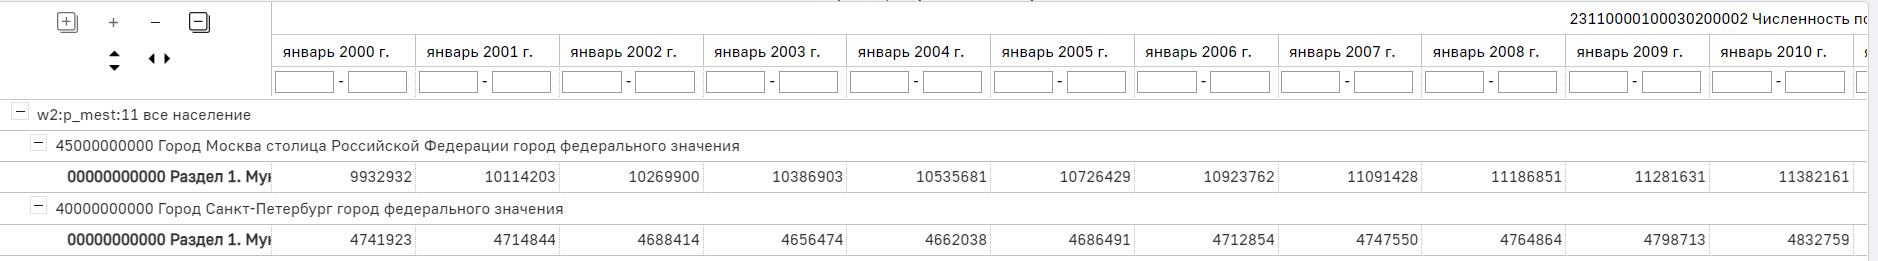
\includegraphics[scale = 0.47]{include/fig/data_rosstat}
	\end{center}
\end{figure}

Всего %\href{https://showdata.gks.ru/report/278928/?&filter_1_0=2000-01-01+00%3A00%3A00%7C-56%2C2001-01-01+00%3A00%3A00%7C-56%2C2002-01-01+00%3A00%3A00%7C-56%2C2003-01-01+00%3A00%3A00%7C-56%2C2004-01-01+00%3A00%3A00%7C-56%2C2005-01-01+00%3A00%3A00%7C-56%2C2006-01-01+00%3A00%3A00%7C-56%2C2007-01-01+00%3A00%3A00%7C-56%2C2008-01-01+00%3A00%3A00%7C-56%2C2009-01-01+00%3A00%3A00%7C-56%2C2010-01-01+00%3A00%3A00%7C-56%2C2011-01-01+00%3A00%3A00%7C-56%2C2012-01-01+00%3A00%3A00%7C-56%2C2013-01-01+00%3A00%3A00%7C-56%2C2014-01-01+00%3A00%3A00%7C-56%2C2015-01-01+00%3A00%3A00%7C-56%2C2016-01-01+00%3A00%3A00%7C-56%2C2017-01-01+00%3A00%3A00%7C-56%2C2018-01-01+00%3A00%3A00%7C-56%2C2019-01-01+00%3A00%3A00%7C-56%2C2020-01-01+00%3A00%3A00%7C-56%2C2021-01-01+00%3A00%3A00%7C-56&filter_2_0=127937&filter_3_0=13200%2C13183&filter_4_0=170792%2C173935%2C155852%2C173936%2C155854%2C155855%2C155857%2C204599%2C155858%2C155859%2C155860%2C155861%2C155863%2C155864%2C155865%2C204601%2C204602%2C155866%2C155867%2C155868%2C155869%2C204603%2C155870%2C204604%2C155871%2C155872%2C155873%2C155874%2C155875%2C155876%2C155877%2C155878%2C155879%2C155880%2C155881%2C155882%2C155883%2C204607%2C155884%2C204609%2C204610%2C211936%2C204611%2C204612%2C155886%2C155887%2C155888%2C155889%2C155890%2C155891%2C155892%2C155893%2C155894%2C155895%2C155896%2C155897%2C155898%2C155899%2C155900%2C155901%2C155902%2C155903%2C211937%2C209086%2C173937%2C155904%2C170794%2C155905%2C155906%2C155907%2C155908%2C204616%2C155909%2C204617%2C155910%2C155911%2C155912%2C155913%2C155914%2C155915%2C155916%2C155917%2C155918%2C155919%2C155920%2C155921%2C155922%2C155923%2C155924%2C155925%2C155926%2C204620%2C155927%2C155928%2C204621%2C155929%2C155930%2C155931%2C155932%2C155933%2C155934%2C155935%2C204623%2C155936%2C155937%2C204624%2C155938%2C155939%2C155940%2C155941%2C155942%2C155943%2C155944%2C155945%2C155946%2C155947%2C155948%2C155949%2C155950%2C155951%2C155952%2C155953%2C155954%2C155955%2C155956%2C155957%2C204628%2C204629%2C155958%2C204630%2C155959%2C204631%2C204632%2C204633%2C204634%2C204635%2C155960%2C155961%2C155962%2C155963%2C204637%2C155964%2C155965%2C155966%2C155967%2C155968%2C155969%2C155970%2C155971%2C155972%2C155973%2C155974%2C204639%2C155975&rp_submit=t}
\href{https://showdata.gks.ru/finder/descriptors/278928}{Росстат} выделяет нам 6 строчек, из которых нужные нам -- 4ая и 6ая.

Открываем Pycharm (Visual Studio Code) и создаем .py-файл. Перво-наперво подключаем нужные нам библиотеки и модули при помощи функции \textit{import}:

\begin{figure}[H]
	\begin{center}
		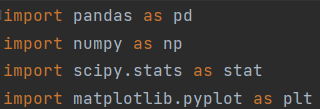
\includegraphics{include/fig/import}
	\end{center}
\end{figure}

Pandas нужен для чтения .xlsx-файла и дальнешей работы с данными; Numpy -- для работы с массивами и вычислениями основным статистик; модуль stats из библиотеки Scipy позволяет вычислять некоторые иными статистики, которых нет в Numpy; и, наконец, модуль pyplot для рисования графиков. Приписка \textit{... as ...} в каждой строчке упрощает обращение к библиотекам -- теперь нет необходимости писать её длинное название, достаточно лишь написать сокращение, которое мы сами можем выбрать.

Далее следует скачать таблицу и поместить её в одну папку с .py-файлом. Для простоты я переименовал её в "moscow\_spb.xlsx". Таким образом, воспользуемся функцией из Pandas для чтения .xlsx-файла:

\begin{figure}[H]
	\begin{center}
		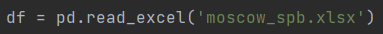
\includegraphics{include/fig/readexcel}
	\end{center}
\end{figure}

Теперь мы можем посмотреть, что внутри переменной df.

\begin{figure}[H]
	\begin{center}
		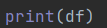
\includegraphics{include/fig/printdf}
	\end{center}
\end{figure}

И мы получим:

\begin{figure}[H]
	\begin{center}
		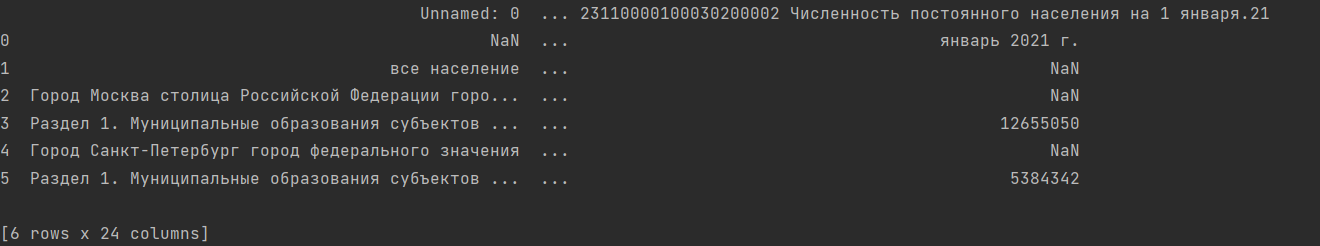
\includegraphics[scale=0.65]{include/fig/print}
	\end{center}
\end{figure}

Да, он не вывел нам всю таблицу, но можно увидеть, что сейчас в датафрейме 6 строк и 24 колонки. Изначально мы уже определили, что нам нужно 2 строчки, а период с 2000 по 2021 составляет 22 значения. Соответственно, нам необходимо "почистить" эти данные.

Со строчками мы определились выше -- 4ая и 6ая, а с колонками всё иначе. Первые две колонки содержат ненужные индексы, а их названия слишком громоздки. Программно это выглядит следующим образом:

\begin{figure}[H]
	\begin{center}
		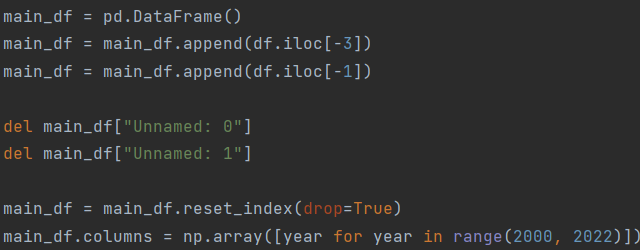
\includegraphics{include/fig/maindf}
	\end{center}
\end{figure}

Сначала мы создаем пустой датафрейм, куда мы положим нужные нам столбцы и строки. Затем мы добавляем нужную строку при помощи метода .append. То, что находится в скобках после .append -- это то, что мы добавляем в main\_df. Метод .iloc позволяет обращаться к строкам датафрейма по индексу. Этот индекс начинается с нуля, то есть, df.iloc[0] выдаст нам первую строчку, df.iloc[1] -- вторую и т.д.. Однако массивы в Python позволяют принимать отрицательные значения, что равносильно "проходу по массиву" в обратную сторону. Это значит, что df.iloc[-1] выдаст последнюю строку, а df.iloc[-3] - третью с конца. Итак, строки добавлены.

Далее мы определили, что первые две колонки содержат незначащие индексы и подписи, поэтому при помощи функции del эти колонки последовательно удаляются. Так как у них не было названия, к ним можно обратиться как "Unnamed: 0" и "Unnamed: 1" соответственно.

Если мы посмотрим на наш датафрейм сейчас, то увидим громоздкие названия столбцов и неверые индексы у строк. К названиям столбцов можно обратиться при помощи метода .columns, а присвоение чего-либо соизмеримого их просто переименует. Так показано, что мы добавляем массив (array), в котором последовательно указаны все года (все целые значения), принадлежащие полуинтервалу $\left[2000, 2022\right)$. У любого датафрейма также есть возможность сбросить по умолчанию нумерацию строк -- .reset\_index(drop=True).

"Очищенные" данные выглядят следующим образом:

\begin{figure}[H]
	\begin{center}
		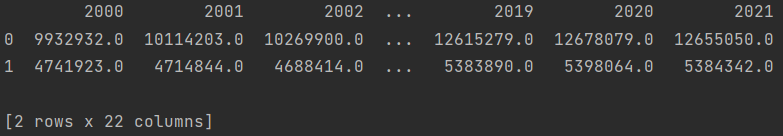
\includegraphics{include/fig/cleardf}
	\end{center}
\end{figure}

Первый город -- Москва, второй -- Санкт-Петербург. То есть, наша задача сводится к тому, чтобы пройти датафрейм построчно, описать данные и нанести их на график.

Метод .iterrows() выдает нам 2 значения -- индекс строки и саму строку. Таким образом, запустив цикл, мы можем "пройтись" по всем строкам. То есть,

\begin{figure}[H]
	\begin{center}
		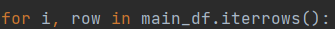
\includegraphics{include/fig/iterrows}
	\end{center}
\end{figure}

На каждой из двух итераций в переменную row будет записан массив с 22мя значениями. Этого хватит, чтобы найти разные статистики.

\begin{figure}[H]
	\begin{center}
		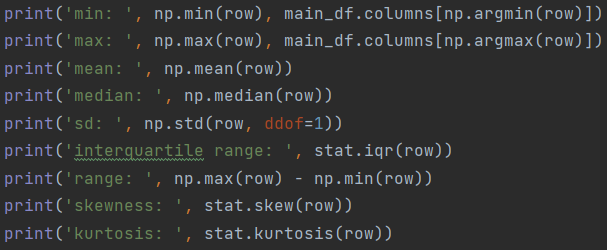
\includegraphics{include/fig/describe}
	\end{center}
\end{figure}

По порядку:
\begin{itemize}
	\item min - минимум;
	\item max - максимум;
	\item mean - среднее;
	\item median - медиана;
	\item sd (std) - стандартное отклонение;
	\item interquartile range (iqr) - интерквартильный размах;
	\item range - размах;
	\item skewness (skew) - коэффициент асимметрии;
	\item kurtosis - эксцесс.
\end{itemize}

\newpage

 % Элементы анализа данных
	\newpage
\addcontentsline{toc}{section}{Методы математической статистики}
\section*{Методы математической статистики}

\addcontentsline{toc}{subsection}{Выборка. Описательная статистика}
\subsection*{Выборка. Описательная статистика}

\addcontentsline{toc}{subsection}{Точечные оценки}
\subsection*{Точечные оценки. Свойства и методы построения}

\newpage
\addcontentsline{toc}{subsection}{Доверительные интервалы}
\subsection*{Доверительные интервалы}

\addcontentsline{toc}{subsection}{Статистические гипотезы. Параметрические критерии}
\subsection*{Статистические гипотезы. Параметрические критерии}

\addcontentsline{toc}{subsubsection}{Критерии о параметрах нормального распределения}
\subsubsection*{Критерии о параметрах нормального распределения}

\addcontentsline{toc}{subsubsection}{Критерии о параметрах нормального и биномиального распределений}
\subsubsection*{Критерии о параметрах нормального и биномиального распределений}

\addcontentsline{toc}{subsection}{Критерии однородности}
\subsection*{Критерии однородности}

\addcontentsline{toc}{subsubsection}{Параметрические критерии однородности}
\subsubsection*{Параметрические критерии однородности}

\addcontentsline{toc}{subsubsection}{Непараметрические критерии однородности}
\subsubsection*{Непараметрические критерии однородности}

\addcontentsline{toc}{subsubsection}{Однофакторный дисперсионный анализ}
\subsubsection*{Однофакторный дисперсионный анализ}

\addcontentsline{toc}{subsection}{Критерии согласия. Таблицы сопряженности}
\subsection*{Критерии согласия. Таблицы сопряженности}

\addcontentsline{toc}{subsubsection}{Критерий согласия хи-квадрат и Колмогорова}
\subsubsection*{Критерий согласия хи-квадрат и Колмогорова}

\addcontentsline{toc}{subsubsection}{Критерий нормальности}
\subsubsection*{Критерий нормальности}

\addcontentsline{toc}{subsubsection}{Таблицы сопряженности}
\subsubsection*{Таблицы сопряженности}

\addcontentsline{toc}{subsection}{Регрессионный анализ}
\subsection*{Регрессионный анализ}

\addcontentsline{toc}{subsubsection}{Множественная линейная регрессия}
\subsubsection*{Множественная линейная регрессия}

\addcontentsline{toc}{subsubsection}{Корреляционный анализ}
\subsubsection*{Корреляционный анализ}
 % Методы математической статистики
	\newpage
\addcontentsline{toc}{section}{Обзор библиотек Python}
\section*{Обзор библиотек Python}

\addcontentsline{toc}{subsection}{Pandas}
\subsection*{Pandas}

\begin{enumerate}
	\item Индексирование, манипулирование, переименование, сортировка, объединение фрейма данных;
	\item Обновить, добавить, удалить столбцы из фрейма данных;
	\item Восстановить недостающие файлы, обработать недостающие данные или NAN;
	\item Построить гистограмму или прямоугольную диаграмму.
\end{enumerate}

\addcontentsline{toc}{subsection}{Numpy}
\subsection*{NumPy}

\begin{enumerate}
	\item Основные операции с массивами: добавление, умножение, срез, выравнивание, изменение формы, индексирование массивов;
	\item Расширенные операции с массивами: стековые массивы, разбиение на секции, широковещательные массивы;
	\item Работа с DateTime или линейной алгеброй;
	\item Основные нарезки и расширенное индексирование в NumPy Python.
\end{enumerate}

\addcontentsline{toc}{subsection}{SciPy}
\subsection*{SciPy}

\begin{enumerate}
	\item Математические, научные, инженерные вычисления;	
	\item Процедуры численной интеграции и оптимизации;
	\item Поиск минимумов и максимумов функций;
	\item Вычисление интегралов функции;
	\item Поддержка специальных функций;
	\item Работа с генетическими алгоритмами;
	\item Решение обыкновенных дифференциальных уравнений.
\end{enumerate}

\addcontentsline{toc}{subsection}{Matplotlib}
\subsection*{Matplotlib}

\begin{enumerate}
	\item Линейные диаграммы;
	\item Точечные диаграммы;
	\item Диаграммы с областями;
	\item Столбцовые диаграммы и гистограммы;
	\item Круговые диаграммы;
	\item Диаграммы «стебель-листья»;
	\item Контурные графики;
	\item Поля векторов;
	\item Спектрограммы.
\end{enumerate}

\addcontentsline{toc}{subsection}{Seaborn}
\subsection*{Seaborn}

\begin{enumerate}
	\item Определять отношения между несколькими переменными (корреляция);
	\item Соблюдать качественные переменные для агрегированных статистических данных;
	\item Анализировать одномерные или двумерные распределения и сравнивать их между различными подмножествами данных;
	\item Построить модели линейной регрессии для зависимых переменных;	
	\item Обеспечить многоуровневые абстракции, многосюжетные сетки.
\end{enumerate} % Обзор библиотек Python для проведения анализа данных и моделирования
	\newpage
\addcontentsline{toc}{section}{Библиотеки Python для проведения анализа данных и моделирования}
\section*{Библиотеки Python для проведения анализа данных и моделирования}

% TODO: Уточнить, что тут % Основы R
	\newpage
\addcontentsline{toc}{section}{Основы R}
\section*{Основы R} % Проведение анализа в R

\end{document}